
\documentclass[]{article}
\voffset=-1.2cm
\oddsidemargin=0.0cm
\textwidth = 480pt
\usepackage[utf8]{inputenc}
\usepackage[english]{babel}
\usepackage{framed}
\usepackage{graphicx}
\usepackage{enumerate}% http://ctan.org/pkg/enumerate
\usepackage{multicol}
\usepackage{amsmath}
\usepackage{amssymb}

\usepackage{eurosym}
\usepackage{vmargin}
\usepackage{amsmath}
\usepackage{graphics}
\usepackage{epsfig}
\usepackage{subfigure}
\usepackage{fancyhdr}
\usepackage{listings}
\usepackage{framed}







\begin{document}

\begin{enumerate}
The probability distribute of discrete random variable $X$ is tabulated below. There are 5 possible outcome of $X$, i.e. 1, 2, 3, 4 and 5.
\begin{center}
\begin{tabular}{|c||c|c|c|c|c|}
\hline
$x_i$  & 1 & 2 & 3 & 4 & 5  \\\hline
$p(x_i)$ & 0.30 & 0.20 & 0.20 & 0.10 & 0.20 \\
\hline
\end{tabular}
\end{center}

\begin{itemize}
%\item[a.] (1 Mark) Compute the value of $k$.
\item[(a)] (2 Mark) What is the expected value of X?
\item[(b)] (2 Mark) Compute the value of $E(X^2)$
\item[(c)] (2 Mark) Compute the variance of $X$.
\end{itemize}
%-----------------------------------%

\item For the following sample of numbers, calculate the following:\\[0.2cm]
	{\bf(a)} Mean. \quad {\bf(b)} Median. \quad {\bf(c)} Standard deviation. \quad {\bf(d)} Inter-quartile range.
	
		\begin{center}
			\begin{tabular}{|cccccccccc|}
				\hline
				&&&&&&&&&\\[-0.4cm]
				2 & 4 & 2 & 1 & 5 & 3 & 0 & 4 & 1 & 8 \\
				\hline
			\end{tabular}
		\end{center}



\end{enumerate}

	
	%==================================================================%
	\subsection*{Question 1A : Introductory Definitions}

	


	
	\subsection*{Question 5 : SPSS Output}
%	\begin{figure}[h!]
%		\centering
%		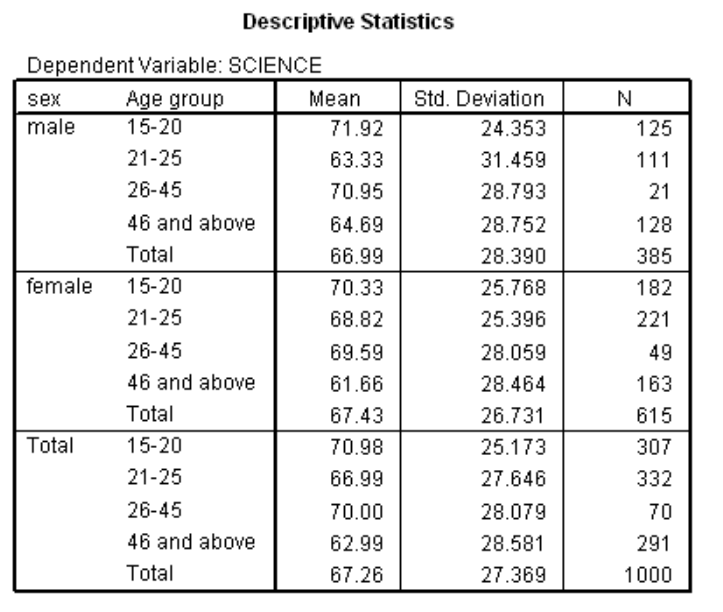
\includegraphics[width=0.65\linewidth]{images/SPSS-Week1}
%	\end{figure}
	\begin{enumerate}
		\item What is the mean Science score for all Males?
		\item What it the mean Science score for all Females?
		\item What is the mean Science score for everybody in the study?
		\item How many respondents are there altogether?
		\item How many people are in the 15-20 age group altogether?
		\item Which Age group has the highest Score?
		%	\item What is the smallest age group in the sample?
	\end{enumerate}
	
\section*{Probability Distributions}


\begin{itemize}
	\item The discrete uniform distribution
	\item The continuous uniform distribution
	\item The binomial disribution
	\item The poisson distribution
	\item The exponential distribution
	\item the Normal distribution
\end{itemize}



%\begin{enumerate}
%	%--Distributions
%	
%	
%	
%	
%	\item uniform - The lower and upper bounds are 13cm and 21cm respectively.
%	
%	\item A computer server breaks down, on average, once every three months.
	\begin{itemize}
		\item What is the probability that the server breaks down three times in a quarter?
		\item What is the probability that a server breaks down exactly five times in one year?
	\end{itemize}
	
	
	

%A charity believes that when it puts out an appeal for charitable donations the donations it receives 
%will normally distributed with a mean 50 and 
%
%standard deviation €6, and
%
% it is assumed that donations will be independent of each other.
%	
%\begin{itemize} 
%\item Find the probability that the first donation it receives will be less than€40.
%
%\item Compute the probability that it will be between €40and €45.
%\item Compute the value $x$ such that 5\% of donations are more than €$x$.
%\end{itemize}
%	


\section{KB Tutorial 2}

\subsection*{Question 4}
Consider a RAID (redundant array of inexpensive disks) system where multiple hard disks are used simultaneously.\\[0.2cm]
Let's assume that we have two hard disks that work \emph{independently} of each other. Define the events $H_1 =$ ``hard disk one works'' and $H_2 =$ ``hard disk two works'' and also assume that $\Pr(H_1) = \Pr(H_2) = 0.9$.\\ \smallskip
\begin{itemize}
	\item RAID-0 is a system which increases performance but only works if \emph{both} hard disks work.
	\item RAID-1 is a system which does not increase performance but still works with only one working hard disk.
\end{itemize}

{\bf(a)} Calculate $\Pr(\text{RAID-0 works})$ and $\Pr(\text{RAID-0 fails})$. \\[0.3cm] \quad {\bf(b)} Calculate $\Pr(\text{RAID-1 works})$ and $\Pr(\text{RAID-1 fails})$. \quad {\bf(c)} Calculate $\Pr(H_1^c)$ and $\Pr(H_2^c)$. \\[0.3cm]
\quad {\bf(d)} Cheap hard disks exist with $\Pr(H) = 0.6$. Consider a RAID-1 system with 3 of these hard disks - calculate $\Pr(\text{RAID-1 fails})$ in this case. \\[0.3cm] \quad {\bf(e)} In part (a) we found that $\Pr(\text{RAID-1 fails}) = 0.01$. How many cheap disks would be required to match this level of reliability?




%-----------------------------------------------------------------------------------------------------------%
\newpage
\section*{MA4603 and MA4505 Tutorial 2 (Week 3)}
Remark : No SPSS related questions this week 



\section{Tutorial C - Probability}	
\subsection*{Question 1}
Assume that there are three different routes to get to a particular location: $R_1$, $R_2$ and $R_3$. You take $R_1$ 75\% of the time, $R_2$ 20\% of the time and $R_3$ the rest of the time. If you take $R_1$, there is a 90\% chance that you will be on time; if you take $R_2$, there is a 50\% chance that you will be on time and, if you take $R_3$, there is a 70\% chance that you will be on time. \\[0.1cm]
Let $T$ represent on time.\\[-0.2cm]

{\bf(a)} If $T$ represents ``on time'', what notation would we use for ``late''? \quad {\bf(b)} What is the value of $\Pr(R_1 \cap R_2)$? \quad {\bf(c)} Calculate the probability of being on time. \quad {\bf(d)} \emph{Given that} you \emph{are} on time, calculate the probabilities of having used each of the routes. \quad {\bf(e)} Given that you are late, what is the probability that you used $R_1$?









\subsection*{Question 4}
Let $X \sim \text{Exponential}(\lambda=0.02)$. Calculate the following:\\[-0.2cm]

{\bf(a)} $\Pr(\,\overline{\!X} > 55)$ in a group of 100. \quad {\bf(b)} $\Pr(\,\overline{\!X} < 53)$ in a group of 40. \quad {\bf(c)} The value of $\bar x$ such that $\Pr(\,\overline{\!X} > \bar x) = 0.1$ when $n=65$. \quad {\bf(c)} The value of $n$ if $\Pr(\,\overline{\!X} < 49) = 0.1$.



\section{KB Tutorial 3}
\subsection*{Question 1}
Assume that there are three different routes to get to a particular location: $R_1$, $R_2$ and $R_3$. You take $R_1$ 75\% of the time, $R_2$ 20\% of the time and $R_3$ the rest of the time. If you take $R_1$, there is a 90\% chance that you will be on time; if you take $R_2$, there is a 50\% chance that you will be on time and, if you take $R_3$, there is a 70\% chance that you will be on time. \\[0.1cm]
Let $T$ represent on time.\\[-0.2cm]

{\bf(a)} If $T$ represents ``on time'', what notation would we use for ``late''? \quad {\bf(b)} What is the value of $\Pr(R_1 \cap R_2)$? \quad {\bf(c)} Calculate the probability of being on time. \quad {\bf(d)} \emph{Given that} you \emph{are} on time, calculate the probabilities of having used each of the routes. \quad {\bf(e)} Given that you are late, what is the probability that you used $R_1$?






\section{KB tutorial 4}

\subsection*{Question 1}
You develop a random number generater which assigns a value to the random variable $X$ according to the following probability distribution:
\begin{center}
	\begin{tabular}{|c|ccccc|}
		\hline
		&&&&&\\[-0.4cm]
		$x$ & 0.0 & 0.5 & 1.0 & 2.0 & 3.0 \\
		\hline
		&&&&&\\[-0.4cm]
		$\Pr(X=x)$ & $0.4$ & $0.2$ & $0.15$ & $0.15$ & $?$ \\[0.1cm]
		\hline
		\multicolumn{6}{c}{}\\
	\end{tabular}
\end{center}

{\bf(a)} What is value the value of $\Pr(X = 3.0)$? \quad {\bf(b)} Calculate $E(X)$ and $Sd(X)$. \quad {\bf(c)} You produce a gambling game where the player wins (in euro) the value of $X$ generated, e.g., if a $2.0$ appears, \euro{2} is won. How much should you charge for a play of this game so that that \emph{you} (the programmer) make a profit of \euro{0.10} on average per game? (i.e., the player \emph{loses} \euro{0.10} on average) \quad {\bf(d)} Using your answer to part (c), determine the probability that you make a profit when somebody plays this game. \quad {\bf(e)} If 10 people play this game, what is the probability that you make a profit 8 times?

\subsection*{Question 2}
You flip three coins. Let $X = $ ``the number of heads'' and $Y = $ ``the number of unique faces''.\\[-0.2cm]

{\bf(a)} What is the sample space for this experiment? \quad {\bf(b)} Construct the \emph{joint distribution} for $X$ and $Y$. \quad {\bf(c)} Based on this joint distribution, construct the \emph{marginal} distribution for $X$ and for $Y$. \quad {\bf(d)} Are $X$ and $Y$ independent? \quad {\bf(e)} Calculate $E(Y)$ and $Sd(Y)$. \quad {\bf(f)} Calculate $\Pr(Y=2\,|\,X=2)$ and interpret its value (compare with $\Pr(Y=2)$).


\subsection*{Question 3}
Let $X =$ ``the attack power of player 1'' and let $Y =$ ``the attack power of player 2''.\\[-0.3cm]

Let the probability distributions for $X$ and $Y$ be:
\begin{center}
	\begin{tabular}{|c|ccc|c|c|ccc|}
		\cline{1-4}\cline{6-9}
		&&&&&&&&\\[-0.4cm]
		$x$ & 0 & 100 & 300 & \qquad\qquad & $y$ & 0 & 80 & 200\\
		\cline{1-4}\cline{6-9}
		&&&&&&&&\\[-0.4cm]
		$\Pr(X=x)$ & $0.2$ & $0.75$ & $0.05$ & & $\Pr(Y=y)$ & $0.1$ & $0.6$ & $0.3$ \\[0.1cm]
		\cline{1-4}\cline{6-9}
		%\multicolumn{9}{c}{}
	\end{tabular}
\end{center}
{\footnotesize(e.g., p1 misses 20\% of the time, deals 100 points of damage 75\% of the time and performs a critical blow 5\% of the time.)}\\[-0.2cm]

{\bf(a)} What is the average attack power of each player? \quad {\bf(b)} If both players have 1000 hit-points, how many attacks does it take for player 1 to defeat player 2 and vice versa? Which player will win on average? \quad {\bf(c)} Let's now assume that player 1 uses his/her \emph{first} turn to cast a spell (and therefore does not attack in this turn). The result of the spell is that player 2 can no longer perform a critical blow, i.e., $\Pr(Y=200) = 0$, \emph{from turn two onwards}. Since setting $p(200) = 0$ leads to $\sum p(y) \ne 1$, assume that the remaining probability ($= 0.3$) is distributed evenly between $p(0)$ and $p(80)$. What is the outcome of the battle now?


\subsection*{Question 4}

You flip a coin 10 times - let $X =$ ``the number of heads''. Using the binomial probability function, calculate the following:\\[-0.2cm]

{\bf(a)} $\Pr(X = 2)$. \quad {\bf(b)} $\Pr(X = 0)$. \quad {\bf(c)}  $\Pr(X > 2)$. \quad {\bf(d)} $\Pr(X \le 3)$. \quad {\bf(e)} $\Pr(5 \le X \le 7)$.  \quad {\bf(f)} $E(X)$ and $Sd(X)$. \quad {\bf(g)} Using the binomial tables, calculate $\Pr(X \le10)$ in the case where the coin is flipped 20 times. \quad {\bf(h)} If the coin is flipped 50 times, what is $E(X)$?

\subsection*{Question 5}

Repeat Question 4 (a) - (e) but now using the binomial tables.



\subsection*{Question 6}

Let's assume that a sequence of bits (binary numbers) is transmitted and, at the other end, decoded; the decoder has a 10\% chance reading a bit incorrectly (i.e., reading a 0 as 1 or vice versa). Let $X$ be the number of errors in the sequence received (i.e., the decoded sequence). Calculate the probability that there are: \\[-0.2cm]

{\bf(a)} \emph{No} errors in a 20-bit string. \quad {\bf(b)} Less than three errors in a 10-bit string. \quad {\bf(c)} More than 10 errors in (i) a 50-bit string and (ii) a 100-bit string (hint: use tables). \quad {\bf(d)} Calculate the average number of errors in a 100-bit string. Calculate the standard deviation also.


\subsection*{Question 7}
We follow on from Question 6 but now consider the case where, to reduce the probability of error, each bit is sent \emph{three} times and then a ``majority vote'' approach is used to determine the value of each received bit. The following example explains the situation:\\[-0.5cm]
\begin{center}
	\begin{tabular}{ccccc}
		\hline
		&&&&\\[-0.3cm]
		\multirow{2}{*}{Sent} & $0$ & $1$ & $1$ & $0$ \\
		& $\overbrace{000}$ & $\overbrace{111}$ & $\overbrace{111}$ & $\overbrace{000}$ \\[0.2cm]
		\hline
		&&&&\\[-0.3cm]
		\multirow{2}{*}{Received} & $\underbrace{001}$ & $\underbrace{111}$ & $\underbrace{010}$ & $\underbrace{000}$ \\
		& $0$ & $1$ & $0$ & $0$ \\[0.2cm]
		\hline
		%\multicolumn{5}{c}{}
	\end{tabular}
\end{center}
$\Rightarrow$ there is one error in decoding the first $000$, but since the majority result is taken, this bit is correctly identified as a $0$. There are two errors in decoding the second $111$, so this bit is misread as a $0$. It is clear that a character is misread if the decoder makes \emph{two or three errors} in these blocks of three replicates.\\[-0.2cm]

{\bf(a)} Show that sending each bit 3 times reduces the error probability from 10\% to 2.8\%. \quad\\ {\bf(b)} Using this reduced value, $p=0.028$, calculate the probability that there are no errors in a 20-bit string. Compare this result to Q6(a). \quad {\bf(c)} Now assume that each bit is sent 5 times and, again, the majority vote approach is used. Calculate the probability that there are no errors in a 20-bit string in this case. %\quad {\bf(d)} Recalculate the two probabilities from part (c) using the Poisson approximation.

\newpage
\section{KB Tutorial 6}


\subsection*{Question 2}
Consider an $M/M/1$ system with arrivals $X_a \sim \text{Poisson}(\lambda_a=3 \text{ / minute})$ and service time \\$T_s \sim \text{Exponential}(\lambda_s=4 \text{ / minute})$. Calculate the following:\\[-0.2cm]

{\bf(a)} The expected time spent in the system. \quad {\bf(b)} The expected time spent in the queue component. \quad {\bf(c)} The expected number of individuals in the system.  \quad {\bf(d)} The expected number of individuals in the queue component. \quad {\bf(e)} The utilisation factor. \quad {\bf(f)} The probability that an individual spends more than 2 minutes in the system. \quad {\bf(g)} The probability that less than 3 individuals exit the system in a 1 minute period.





\subsection*{Question 3}
Customers arrive to a deli counter at a rate of 12 per hour. On average it takes 3 minutes to serve a customer at this counter. Customers then exit and head to another counter to pay. It takes 1 minute to deal with a customer at this counter. We will assume that arrivals have a Poisson$(\lambda_a)$ distribution and service times have Exponential$(\lambda_{s1})$ and Exponential$(\lambda_{s2})$ distributions respectively (hint: this is a sequence of two $M/M/1$ systems).\\[-0.2cm]

{\bf(a)} What is the average time spent in each sub-system? \quad {\bf(b)} What is the average total time spent in the system? \quad {\bf(c)} How many customers are there (on average) in the system?  \quad \\{\bf(d)} Calculate the utilisation factor for each sub-system. \quad {\bf(e)} What is the average total queueing time? (i.e., total time excluding service time) \quad {\bf(f)} Calculate the probability that at least 20 people exit the shop (i.e., the whole system) in one hour.



\subsection*{Question 4}
{\footnotesize({\bf Note}: this is not a queueing theory question. It is a generalisation of a question which appears on Tutorial2)}\\[0.1cm]
There are two possible routes to a particular location. You take $R_1$ 80\% of the time and $R_2$ 20\% of the time. We assume that travel time has an exponential distribution and, furthermore, the average travel time is 0.25 hours if you take $R_1$ and 0.5 hours if you take $R_2$.\\[-0.2cm]

{\bf(a)} Calculate the probability that the journey takes more than 0.5 hours for each of the routes, i.e., $\Pr(T > 0.5\,|\,R_1)$ and $\Pr(T > 0.5\,|\,R_2)$ respectively. \quad {\bf(b)} Calculate $\Pr(T > 0.5)$. (hint: law of total probability) \quad {\bf(c)} Given that $T>0.5$ hours, what is the probability that you used $R_1$? (i.e., calculate $\Pr(R_1\,|\,T>0.5)$) \quad {\bf(d)} Derive a general expression for $\Pr(R_1\,|\,T>t)$ and evaluate it at $t=0.25$, $t = 1$ and $t = 2$ respectively. Interpret the results.








\end{document}
